%!TEX root = /Users/jakubkonka/Thesis/Thesis.tex
\chapter{FIX:ME Approximating...}
\label{cha:approximation}

\minitoc
\vspace{10mm}

This chapter explores whether an auction format represented by the DMP selling mechanism can be modeled as an asymmetric first-price sealed-bid auction (FPA) with common priors; that is, an auction in which bidders are characterized by different probability distributions sharing a common support. Ideally, if the DMP auction was shown to be a special case of some corresponding common priors auction, then the numerical solution methods presented in Hubbard and Parsch~\cite{HubbardPaarsch2011}, and extensively studied by the economic community, could be employed. Conversely, if the DMP auction format cannot be shown to constitute a special case of the common priors auction, then, provided the expected profits for the bidders in both auction formats differ only slightly, the common priors auction could still effectively be used to approximate the solution to the DMP auction.

\section{Mathematical Description} % (fold)
\label{sec:mathematical_description_approximation}

Following the notation of Chapter~\ref{cha:indirect}, let each bidder $i$ be characterized by the utility function
\begin{equation*}
    u_i(b,c) = \left\{
  \begin{array}{l l}
    b_i-c_i & \;\text{if } b_i < \displaystyle\min_{j\neq i}b_j,\\
    0 & \;\text{if } b_i > \displaystyle\min_{j\neq i}b_j,
  \end{array}\right.
\end{equation*}
where, as before, $b = (b_1,\ldots,b_n)$, and $c = (c_1,\ldots,c_n)$. In the common priors auction, we assume that each bidder $i$ draws their cost from common support across all bidders; i.e., let
\begin{equation*}
  c_i\in [\underline{c}, \bar{c}] \quad\text{for all } i\in N \text{ such that } [\underline{c}, \bar{c}]\subseteq [0, 1].
\end{equation*}

Let $F_i$ be the distribution function of $c_i$ for all $i\in N$. Note that the distribution functions between bidders need not be equal, and hence, we are dealing with an asymmetric FPA.

We further assume that
\begin{assumptions}
\label{ass:assumptions_common_priors_approximation}
Assume that
\begin{enumerate}
  \item $F_i$ is differentiable over $(\underline{c}, \bar{c}]$ with a derivative $f_i$ locally bounded away from zero over this interval;
  \item $F_i$ is atomless; and
  \item $F_i(c)>0$ for all $c\in [\underline{c}, \bar{c}]$ and $i\in N$.
\end{enumerate}
\end{assumptions}
These assumptions correspond to Assumptions~A.1 and Theorem~U.1 in Lebrun~\cite{Lebrun2006}, and, as shown by Lebrun, with these assumptions satisfied, there exists one and only one pure-strategy Bayesian Nash equilibrium where bidders engage in serious bidding; that is, bid at least their cost. Formally,
\begin{proposition}[Characterization of the Equilibrium in Common Priors Setting]
\label{prop:characterization_of_the_equilibrium_in_common_priors_setting_approximation}
Let Assumptions~\ref{ass:assumptions_common_priors_approximation} be satisfied. There exists one and only one pure-strategy Bayesian Nash equilibrium where bidders submit at least their costs. In every such equilibrium, bidder $i\in N$ follows a bid function $b_i$, for all $1\leq i\leq n$ such that its inverse, $c_i\equiv b_i^{-1}$, satisfy the following system of differential equations
\begin{equation*}
  \frac{d}{db}c_i(b) = \frac{1 - F_i(c_i(b))}{f_i(c_i(b))}\left[ \frac{1}{n-1}\sum_{k=1}^n \frac{1}{b-c_k(b)} - \frac{1}{b-c_i(b)} \right]
\end{equation*}
for all $1\leq i\leq n$, with the following lower boundary condition
\begin{equation}
  \label{eq:foc_ode_lower_boundary_approximation}
  c_i(\underline{b}) = \underline{c}
\end{equation}
and the upper boundary condition
\begin{equation}
  \label{eq:foc_ode_upper_boundary_approximation}
  c_i(\bar{c}) = \bar{c}
\end{equation}
for all $1\leq i\leq n$.
\end{proposition}

In effect, Proposition~\ref{prop:characterization_of_the_equilibrium_in_common_priors_setting_approximation} is a special case of Proposition~\ref{prop:characterization_of_the_equilibrium_indirect}. That is, the equilibrium bidding functions still have to satisfy the system of nonlinear ODEs given by Equation~\eqref{eq:foc_ode_indirect}; however, in this case, the lower boundary condition reduces to
\begin{equation*}
  c_i(\underline{b}) = \underline{c},
\end{equation*}
and the upper boundary condition to
\begin{equation*}
  c_i(\bar{c}) = \bar{c},
\end{equation*}
i.e., the bids never exceed the upper extremity of the common support range.

It should be noted that, even though the bidding problem is considerably simpler than the original one discussed in this thesis, it still involves finding the lower bound on bids, and hence, the closed-form solution exists only in a handful of special cases~\cite{Krishna10,HubbardPaarsch2011}.

% section mathematical_description (end)

\section{Numerical Solutions} % (fold)
\label{sec:numerical_solutions}

As already mentioned in the previous chapter, however, the problem can be approximated using numerical methods (see Hubbard and Paarsch~\cite{HubbardPaarsch2011} for an excellent discussion). In this chapter, a common priors auction is approximated using the forward shooting method (FSM), but tailored to the problem at hand. The FSM method was chosen due to its relatively low implementation complexity, and the fact that a similar method was used to solve the DMP bidding problem. Therefore, the numerical solutions to the DMP and common priors auctions should be of comparable quality (in terms of the numerical accuracy).

\subsection{Forward Shooting Method} % (fold)
\label{sub:forward_shooting_method}

To briefly recap, the FSM method was first proposed by Bajari~\cite{Bajari2001a} (cf.~Algorithm~1 in \cite{Bajari2001a}). The method aims at finding the best approximation of the lower bound on bids, $\underline{b}$, by successively picking a value from the feasible interval, $(\underline{c}, \bar{c})$, and verifying whether a numerical solution to the initial value problem

\begin{equation}
  \label{eq:fsm_initial_value_problem_approximation}
  \begin{array}{ll}
     \displaystyle\frac{d}{db}c_i(b) &= \displaystyle\frac{1 - F_i(c_i(b))}{f_i(c_i(b))}\left[ \frac{1}{n-1}\sum_{k=1}^n \frac{1}{b-c_k(b)} - \frac{1}{b-c_i(b)} \right]\\[2ex]
    c_i(\underline{b}) &= \underline{c}
  \end{array}
\end{equation}

for all $i\in N$, lies within a set of permissible functions, $S$, such that every element of that set is a function mapping $[\underline{b}, \bar{c}]$ into $[\underline{c}, \bar{c}]$, it is monotonically increasing everywhere except possibly at $\underline{c}$, and each function value is strictly lower than its argument except possibly at $\bar{c}$; that is,

\begin{equation*}
  S\equiv\left\{s \:\middle\vert\:
  \begin{array}{l}
    s: [\underline{b}, \bar{c}]\to [\underline{c}, \bar{c}],\\
    b_1 < b_2\implies s(b_1) < s(b_2) \text{ for all }b_1,b_2\in [\underline{b}, \bar{c}),\\
    s(b) < b \text{ for all }b\in [\underline{b}, \bar{c})
  \end{array}
  \right\}.
\end{equation*}

The pseudo-code for the FSM is depicted in listing Algorithm~\ref{alg:forward_shooting_method_approximation}. Note that the algorithm is almost identical to the FSM version tailored to the DMP auction (cf.~Algorithm~\ref{alg:forward_shooting_method_indirect}), with only differences being the definition of the set of permissible functions, $S$, and the algorithm's search region delimited by $low$ and $high$ variables. Hence, we omit the discussion of the algorithm and refer the Reader to Section~\ref{sub:forward_shooting_method_indirect}.

\begin{algorithm}
\caption{Forward shooting method (common priors version)}
\label{alg:forward_shooting_method_approximation}
\begin{algorithmic}[1]
\Require{$\epsilon\in (0, \bar{c} - \underline{c}); low, high\in [\underline{c}, \bar{c}]$ such that $low\leq high$}
\Ensure{Approximation to $\underline{b}$}
  \Statex
  \Let{$low$}{$\underline{c}$}
  \Let{$high$}{$\bar{c}$}
  \Statex
  \While{$high-low > \epsilon$}
    \Let{$guess$}{$0.5\cdot(low + high)$}
    \Let{$bids$}{$[guess, \bar{c})$}
    \Let{$(costs_1,\dotsc,costs_n)$}{solve~\eqref{eq:fsm_initial_value_problem_approximation} with initial value $\underline{b} = guess$}
    \StatexIndent[7.5]{evaluated at points $b\in bids$}
    \If{$(bids,costs_i)\in S$ for all $i\gets 1$ to $n$}
      \Let{$high$}{$guess$}
    \Else
      \Let{$low$}{$guess$}
    \EndIf
  \EndWhile
  \Statex
  \Let{$\underline{b}$}{$0.5\cdot(low + high)$}
\end{algorithmic}
\end{algorithm}

Similarly to the implementation of the FSM algorithm for the DMP auction, the approximation results presented in this chapter have been derived using the GNU Scientific Library (GSL) implementation of the Embedded Runge-Kutta-Fehlberg (4,5) method.

% subsection forward_shooting_method (end)

\subsection{Verification} % (fold)
\label{sub:verification}

Before proceeding with the modeling and analysis, the FSM algorithm was tested for correct implementation. The bidding scenario used to verify the algorithm is taken from the Bajari's paper \cite{Bajari2001a}. There are three bidders, and each is characterized by a truncated normal distribution but with different mean and standard deviation parameters (Table~\ref{tab:verification_approximation}). Furthermore, each bidder draws their cost from common range of costs, $c_i\in [2,8]$.

\begin{table}[t]
  \caption{Test bidding scenario}
  \vspace{0.5cm}
  \begin{tabular*}{0.5\columnwidth}[L]{@{\extracolsep{\fill}}r c c}
    \hlx{vhv}
    & \textbf{Mean}, $\mu_i$ & \textbf{Standard deviation}, $\sigma_i$\\
    \hlx{vhv}
    \textbf{Bidder 1} & $4$ & $1.5$\\
    \textbf{Bidder 2} & $5$ & $1.5$\\
    \textbf{Bidder 3} & $6$ & $1.5$\\
    \hlx{vhs}
  \end{tabular*}
  \label{tab:verification_approximation}
\end{table}

Figure~\ref{fig:fsm_common_priors_verification_approximation} depicts the numerically approximated solution to the problem. It is clear that the approximation agrees with that of Bajari's~\cite{Bajari2001a}. Furthermore, in Figure~\ref{fig:fsm_common_priors_verification_sufficiency_approximation}, the numerical solution is verified whether it satisfies the sufficiency condition for an equilibrium; that is, whether the numerically derived bidding strategy for each bidder is a best response to the bidding strategies of the remaining bidders. As expected, the solution satisfies the sufficiency condition, and hence, we conclude that the algorithm was implemented correctly.

\begin{figure}[p!]
  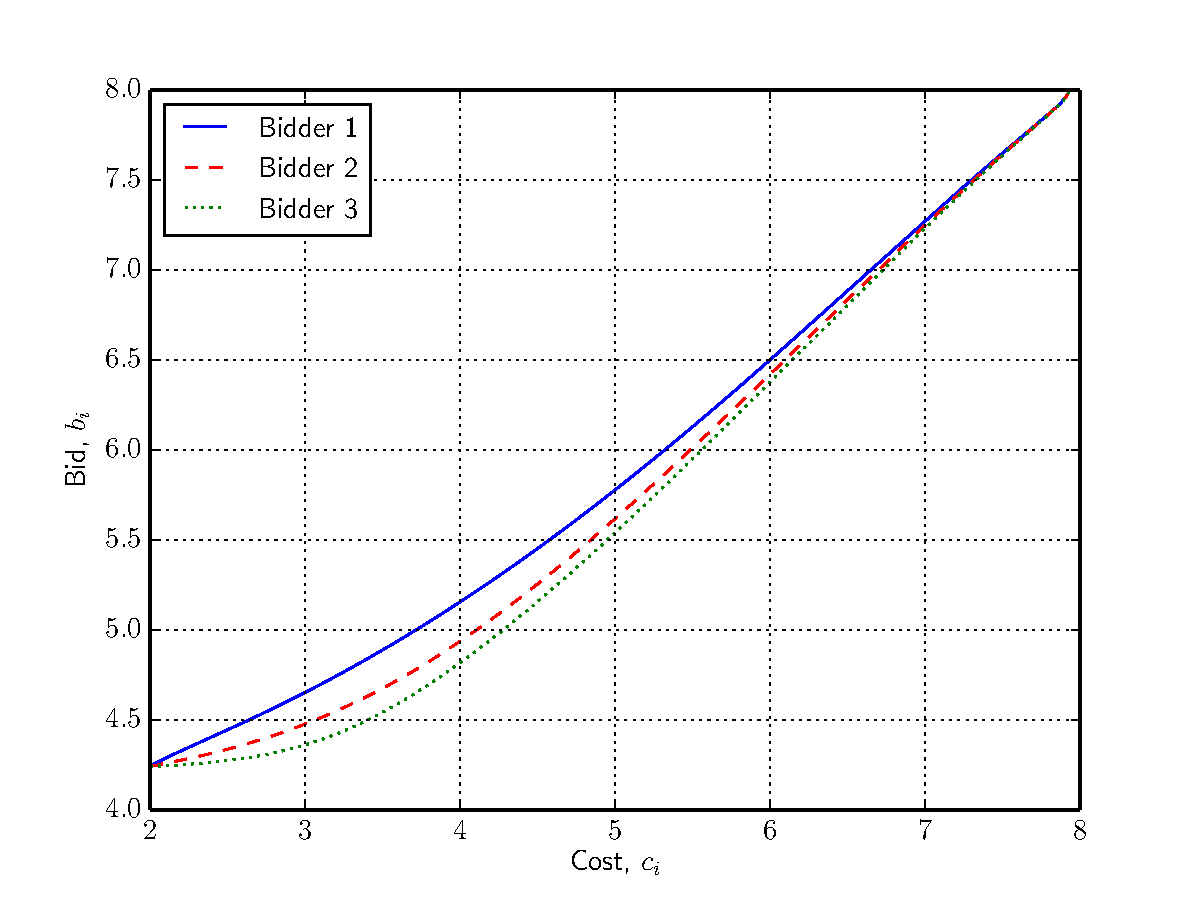
\includegraphics[width=\figsize]{Approximation/Figures/fsm_common_priors_verification}
  \caption{FIX:ME FSM Common Priors verification}
  \label{fig:fsm_common_priors_verification_approximation}
  \vspace{10mm}
  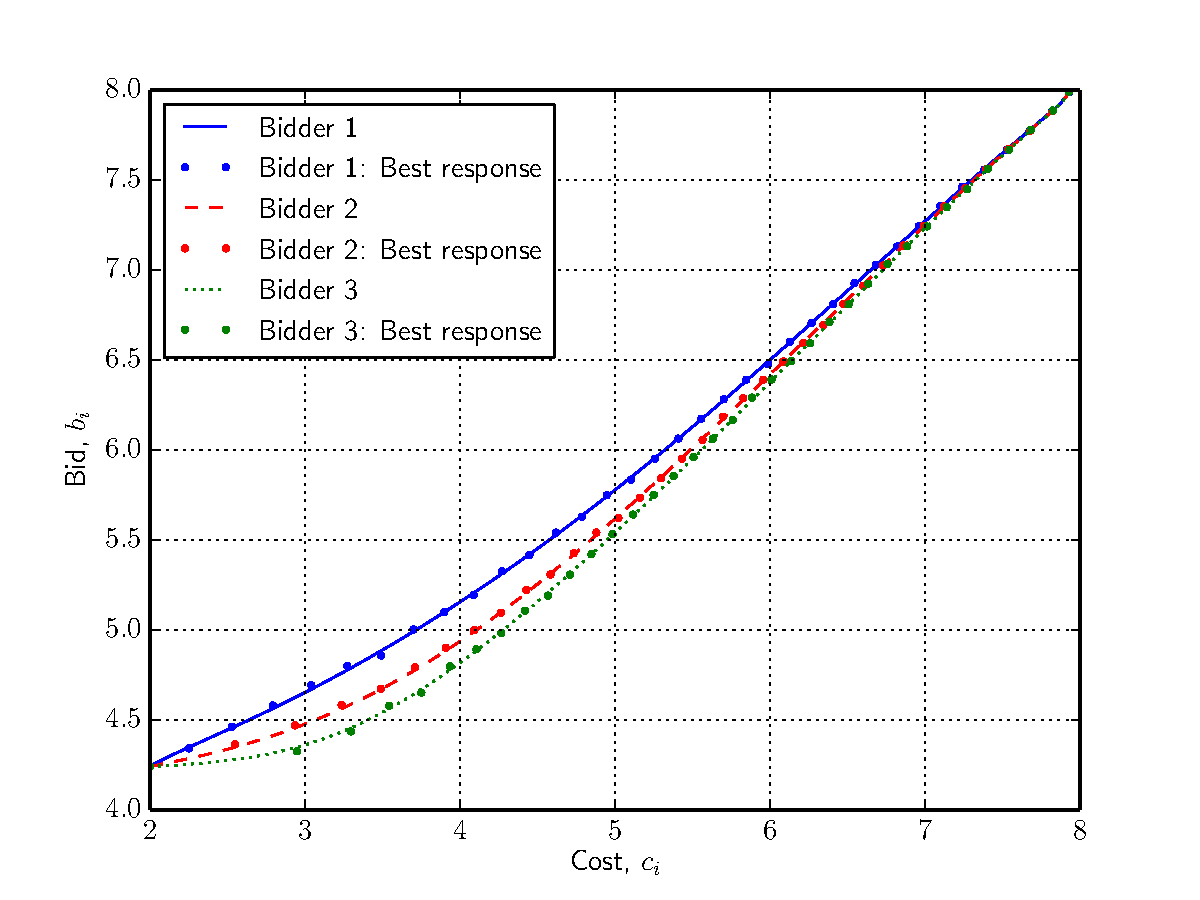
\includegraphics[width=\figsize]{Approximation/Figures/fsm_common_priors_verification_sufficiency}
  \caption{FIX:ME FSM Common Priors verification}
  \label{fig:fsm_common_priors_verification_sufficiency_approximation}
\end{figure}

% subsection verification (end)

% section numerical_solutions (end)

\section{Network Selection Mechanism Cast into Common Priors Setting} % (fold)
\label{sec:network_selection_mechanism_cast_into_common_priors_setting}

% section network_selection_mechanism_cast_into_common_priors_setting (end)

\section{Summary} % (fold)
\label{sec:summary_approximation}

% section summary_approximation (end)
